\chapter{Experiment}
\label{Chapt:experiment}

%\everypar{\looseness=-1}
The experiment of the electron scattering off deuterium nuclei, that provides data for this study, was conducted at JLab Hall B as a part of the ``e1e" run period. A~longitudinally polarized electron beam of 2.039~GeV energy was produced by the Continuous Electron Beam Accelerator Facility (CEBAF) and then scattered off the 2-cm-long liquid deuterium target, which was located in the center of the CEBAF Large Acceptance Spectrometer (CLAS)~\cite{Mecking:2003zu}. This state of the art detector covered a good fraction of the full solid angle and provided efficient registration of the final-state particles originating from the scattering process.





\section{Detector setup}
\label{Sect:detector}

%\everypar{\looseness=-1}
The CLAS design is based on a toroidal magnetic field, which is generated by six superconducting coils arranged around the beamline. The magnetic field bends charged particles toward or away from the beam axis (depending on the particle charge and~the direction of the torus current) but leaves the azimuthal angle essentially unchanged. The magnet coils naturally separate the detector into six areas, the \text{so-called} ``sectors", each functioning as an independent magnetic spectrometer. Each sector includes four sub-detectors: Drift Chambers (DC), \v Cerenkov Counters (CC), Time-of-Flight System (TOF), and Electromagnetic Calorimeters (EC)~\cite{Mecking:2003zu}. A view of the detection system in the direction of the beam (cut through the target region) is given in Fig.~\ref{fig:clas}.


\clearpage
\begin{figure}[htp]
\begin{center}
\framebox{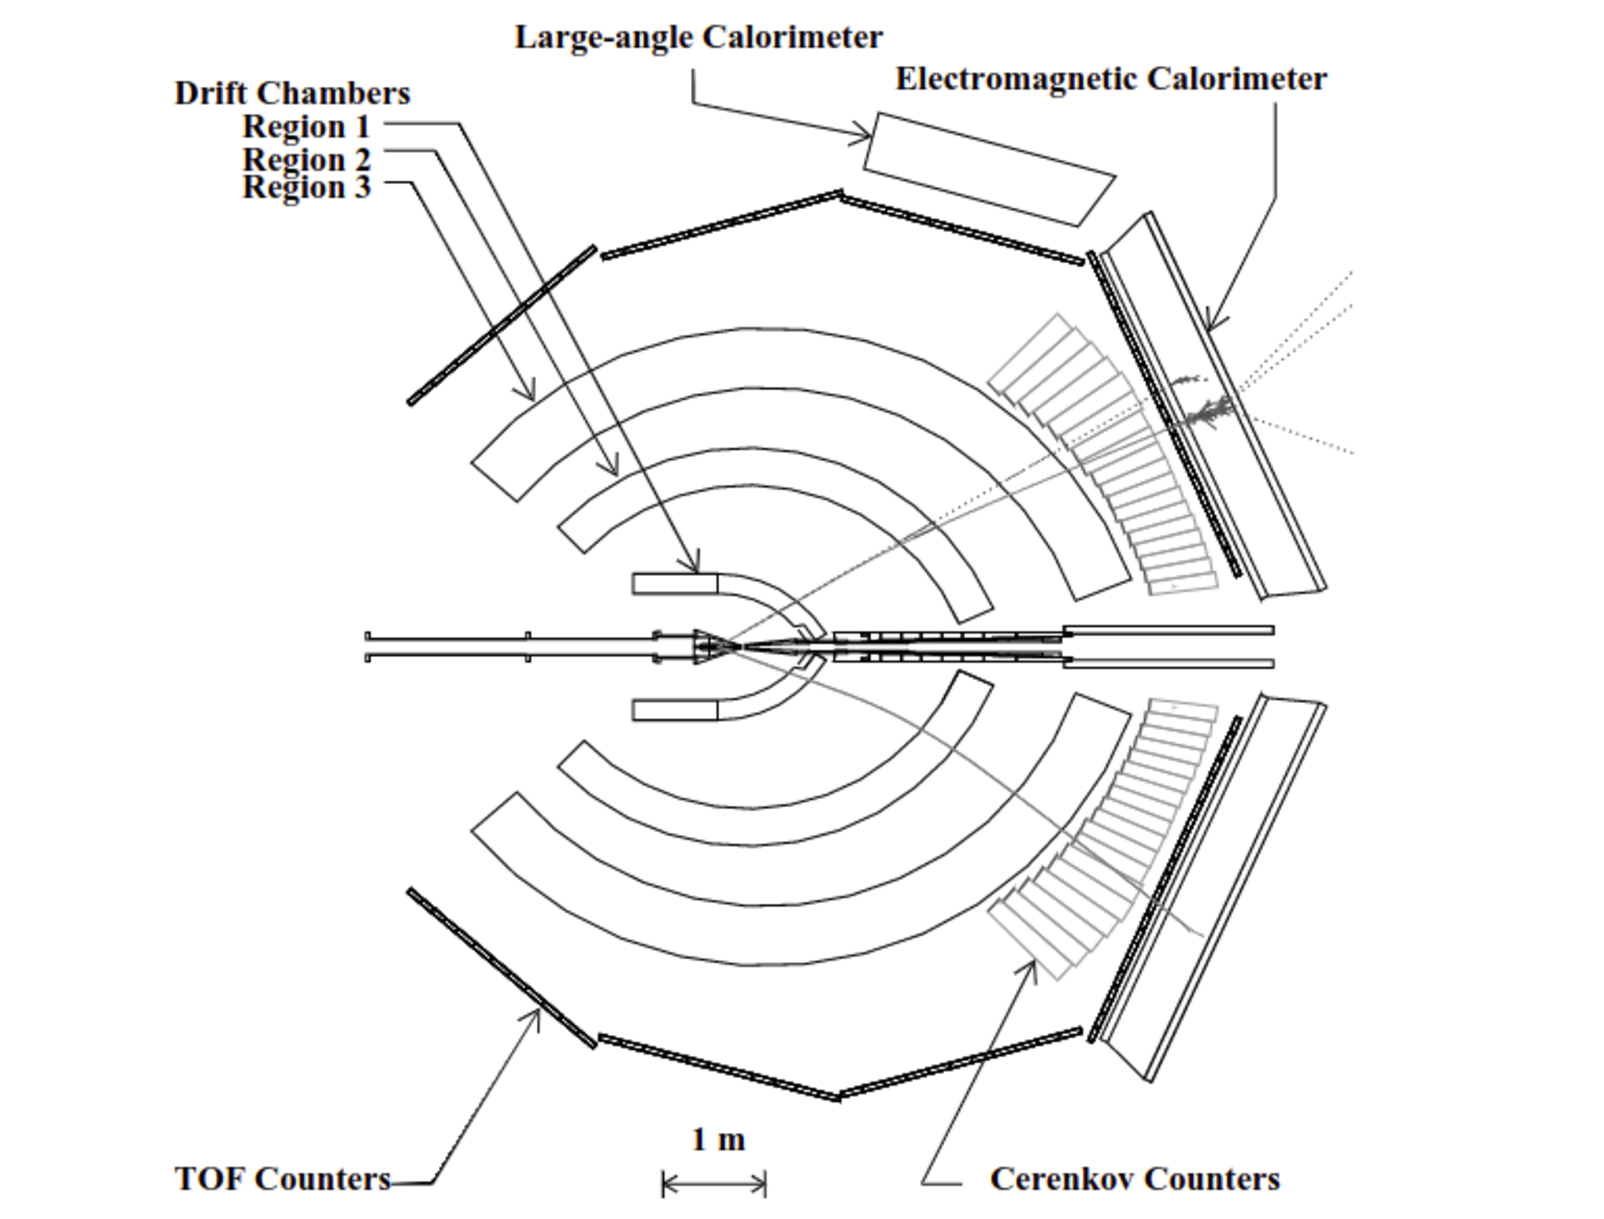
\includegraphics[width=0.8\textwidth]{pictures/experiment/clas2.pdf}}
\caption{\small A schematic top view of the CLAS detector cut along the beam line. Typical photon, electron, and proton tracks (from top to bottom) from an interaction in the target are superimposed on the figure. The figure is taken from Ref.~\cite{Mecking:2003zu}} \label{fig:clas}
\end{center}
\end{figure}
\begin{figure}[!ht]
\begin{center}
\framebox{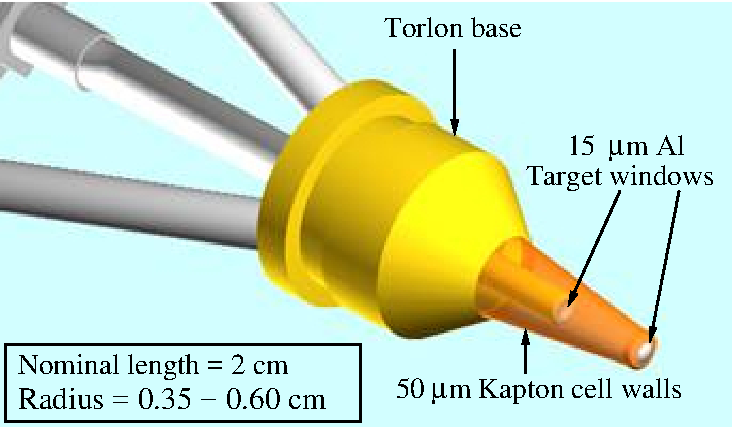
\includegraphics[width=0.8\textwidth]{pictures/experiment/e1e_target_small.pdf}}
\end{center}
\caption{\small The target cell and its support structure used during the ``e1e" run period~\cite{target}. The figure is taken from Ref.~\cite{Fed_paper_2018}. }\label{fig:e1e_target}
\end{figure}


The azimuthal coverage for CLAS is limited only by the magnet coils and approximately 90\% at large angles and 50\% at forward angles~\cite{Amarian:2001zs}. The coverage in the polar angle is from $8^{\circ}\mathrm{}$ to $45^{\circ}\mathrm{}$ for the \v Cerenkov Counters and Electromagnetic Calorimeter and from $8^{\circ}\mathrm{}$ to $142^{\circ}\mathrm{}$ for the Drift Chambers and the Time-of-Flight system.

The Drift Chambers are located within the region of the magnetic field, which bends the trajectories of the charged particles traveling through. The Drift Chambers perform the particle tracking, allowing the determination of the particle momentum from the curvature of its trajectory. Other sub-detectors are located outside the magnetic field region, which means that having left the DC, the charged particles move further along a straight line.

The \v Cerenkov Counters are located right behind the DC and serve the dual function of triggering on electrons and separating electrons from pions~\cite{Adams:2001kk}. 

The TOF scintillators are located radially outside the Drift Chambers and the \v Cerenkov Counters but in front of the Calorimeters~\cite{Smith:1999ii, clas_tof_paddles}. Their alignment and relative positioning with respect to other detector sub-systems is shown in Fig.~\ref{fig:clas}. The Time-of-Flight system measures the time when a particle hits a TOF scintillator, thus allowing for the determination of its velocity. With the help of the particle momentum known from the DC, its mass can then be determined, which means that the particle can be identified.

The main functions of the Electromagnetic Calorimeter are triggering on and detection of electrons at energies above 0.5~GeV, detection of photons at energies above 0.2~GeV (allowing for the $\pi^{0}$ and $\eta$ reconstructions from their $2\gamma$ decays), and detection of neutrons~\cite{Amarian:2001zs}. 

The six CLAS sectors are equipped with a common data-acquisition (DAQ) system that collects the digitized data and stores the information for later off-line analysis.


\newpage
\section{Target setup}
\label{Sect:target}



The target design was specific for the ``e1e" run period~\cite{target}. The setup of the target cell with its support structure is presented in Fig.~\ref{fig:e1e_target}. For this particular part of the ``e1e" run period, the target cell was filled with liquid deuterium.



The conical shape of the target (with the diameter varying from 0.35 to 0.6 cm) serves the purpose of effective extraction of gas bubbles, which are formed in the liquid target content due to the heat that either originates from the beam and/or comes from outside through the target walls. Due to the conical shape, the bubbles are drained upwards and into a wider area of the target thus clearing the beam interaction region and allowing the boiled deuterium to be effectively delivered back to the cooling system to be condensed. 


The interaction region of the target was 2-cm-long. The target cell had 15-$\mu$m-thick aluminum entrance and exit windows. In addition, an aluminum foil was located 2.0 cm downstream of the target. This foil was made exactly to the same specifications as the entry/exit windows of the target cell and served for both the estimation of the number of events that originated in the target windows and the precise determination of the target $z$-position along the beamline. See also Sect.~\ref{Sect:vertex} for more details.

\section{Experimental data}
\label{Sect:data_format}

The measurements are attributed to the ``e1e" run period that lasted from November 2002 until January 2003. This run period included several experiments with different beam energies (1 GeV and 2.039 GeV) and different target cell contents (liquid hydrogen and liquid deuterium). This study is devoted to the experiment conducted with the 2-cm-long liquid deuterium target and a 2.039 GeV polarized electron beam.


All data collected with the CLAS detector is stored in a specific format, which is the BOS format~\cite{BOS:bank,Stepanyan:1999}. The information on the detector response to particles passing through is recorded for each event and sorted into a set of BOS banks. The original BOS files store the data in terms of ``raw" signals (like TDC, ADC). These ``raw" files are then ``cooked" with the reconstruction software (recsis), which converts the detector response to the variables that characterize the events directly, i.e. the particle momentum, the track coordinates, timing, etc. This information is also stored in BOS banks. However, since the cooking process introduces new variables, the structure of the ``cooked" BOS files is different from that for the ``raw" files. The ``cooked" data is stored in various formats including BOS files and ROOT ntuples. In this analysis the latter were used.%\footnote[1]{The location of the data files is provided in App.~\ref{app_code}. The link to the scripts, which were used in the simulation/reconstruction sequence for this analysis is also given there.}.
%ROOT ntuples for the full target runs are stored in /mss/clas/e1e/production/pass1/h10/, while those for the empty target are in /mss/clas/e1e/production/pass1/h10\_emptarg\_d/.
\section{Data analysis using the CLAS software}
\label{Sect:clas_software}

Events corresponding to the investigated reaction $ep(n) \rightarrow e'p'(n')\pi^{+}\pi^{-}$ are distinguished among all other registered events through the event selection procedure, described in detail in Chapter~\ref{Sect:select}. The selected exclusive events,  however, represent only a part of the total number of events produced in the reaction, while the remainder were not registered due to (i) geometrical holes in the detector acceptance and (ii) less than 100\% efficiency of particle detection within the detector acceptance. Therefore, to extract the reaction cross sections, the experimental event yield should be adjusted for the geometric acceptance and detection efficiency, thus accounting for the lost events.

%\footnote[2]{More details on the efficiency evaluation can be found in Sect.~\ref{Sect:eff_eval}.}

In order to determine the overall detector efficiency, a Monte Carlo simulation is typically performed. In this analysis, double-pion events are generated with TWOPEG-D, which is an event generator for the double-pion electroproduction off a moving proton~\cite{twopeg-d}. These events are hereinafter called ``generated" events. 

The generated events are passed through a standard multi-stage procedure of simulating the detector response~\cite{Mecking:2003zu}. At the first stage the interaction of the generated events with the CLAS detector is simulated. For this purpose, the GSIM package (GEANT SIMulation) is used. GSIM incorporates information about the detector geometry and materials with their electromagnetic properties, magnetic fields, target material and geometry, etc. It  propagates all the particles through the CLAS detector from the vertex produced by the event generator and provides the detector response in terms of the same ``raw" signals as the actual CLAS detector does.

Although the GSIM package includes all the detector geometry and properties, it still does not properly reproduce the resolution of the drift chambers and the TOF system. For that reason the GSIM Post Processor (GPP) is used to better match the resolution as well as to include the effects of a less-than-perfect detector response (due to broken drift wires, problematic phototubes, etc.). The latter effects are unique for a particular run period, and therefore the information on the detector imperfections is usually provided along with the data files to be then used in the GPP. Meanwhile, the GPP parameters intended to adjust the resolution (DC and TOF smearing factors) are typically determined individually during a particular analysis as the resolution depends on the kinematics and hence on the experimental conditions. This analysis employs the same values of the resolution related GPP parameters as the study~\cite{Fed_an_note:2017,Fed_paper_2018} in which the double-pion cross sections off the free proton are measured under the same experimental conditions.



At the final stage, GPP output files are ``cooked" using the same reconstruction software that was used for the real data (recsis). Events that survive after the ``cooking" process are hereinafter called ``reconstructed" Monte Carlo events. They are analyzed in the same way as real experimental events. 



